% University of Leeds PhD thesis style -- modifications to the report style
% This is unofficial so you should always double check against the
% Registrar's office rules
% See http://library.stanford.edu/research/bibliography-management/latex-and-bibtex
% 
% Example of use below
% See the suthesis-2e.sty file for documentation
%
\documentclass{report}
\usepackage{suthesis-2e}
\dept{Electronic and Electrical Engineering}

\usepackage{hyperref}
\usepackage{graphicx}

\begin{document}
\title{CENTRALISED CONTROL ALGORITHMS FOR SMART GRID OPERATION}
\author{Jialeng Guo}
%\principaladviser{John Parker}
%\firstreader{John Green}
%\secondreader{John BigBooty}
%\thirdreader{Jane Supernumerary} %if needed
%\fourthreader{Severus Snape} %if needed

\beforepreface
\prefacesection{Abstract}
Maintaining the frequency at the nominal value in the grid is one of the most elusive and long-standing challenges in smart grids. This project tackles the problem of  frequency changes: how to design an algorithm to build a centralised Secondary Frequency Control (SFC) and to analyse the performance of the gird. On one hand, we think that our SFC algorithm can maintain the frequency. On the other hand, we would need an efficient and concise strategy to analyse the performance of the system if we want to build an optimal controller to ensure that the frequency of the electricity network is always restored to its nominal value when disturbances occur in the system.\\

In this project, we focus on PI Control: the most common control algorithm by far and the standard algorithm in SFC. Compared to traditional grids without SFC, this algorithm have proven to be more effective in maintaining the frequency.\\

This project consists of two parts. In the first part, we aim to understand the physical theory behind SFC and PI control and present our efforts at building effective SFC models.\\

In the second part of this project, we test our algorithm in RAMSES based on Nordic Grid scenario. In particular, 1) how we test our system in a low time delay; 2) how we analyse the impact of different time delays; and 3) how we analyse the impact of generator size and 4) how we test Emergency Control and analyse the impact of time delays.\\

\prefacesection{Acknowledgments}
A special thank to my supervisor Dr Petros Aristidou. He always has a very insightful, high-level view about the field while he is also uncommonly detail oriented and understands the nature of the problems very well. More importantly, Dr Aristidou is an extremely caring and supportive supervisor that I could not have asked for more.\\

Collaboration is a big lesson that I learned, and also a precious part of my undergraduate stage. I thank Sultan Alghamdi. He never reserved his minds when I tried to seek his help. I am glad that my research can help part of his doctoral subject. It was a very unique and rewarding experience for me.\\

I would like to thank Dr Zoran Ikonic. His passionate lecture (ELEC2540 Control Systems) and impressive experiment last year depended my understanding of PI control.\\

I would like thank Walter Roberson from MATLAB for helping me find the clue to solve the problem with plotting a 3D triangle surface plot without a clearly relationship between variables.\\

Lastly, I would like to thank other staffs and my fellow schoolmates in School of Electronic and Electrical Engineering, without them, this project would not be finished smoothly: Anna de Jong, Nathan Smith, Zikang Qian and Al Dabashi.\\



\afterpreface


\chapter{Introduction}
\section{Motivation}
The motivation for doing this project contains a vision of restructuring and sustainability of energy in the future.
\subsection{Problems in the Grid}
\subsubsection{A. Energy Crisis}
The energy crisis is one of the most essential and critical crises in the 21st century.

Nowadays, non-renewable resource still consists of a large proportion in the energy system. Non-renewable resource, or finite resource, is depleting. Although we might not meet the complete depletion of non-renewable resources in the future 50 years, based on Hotelling’s "Economics of Exhaustible Resources", David Ricardo proposed that as the historical production stock accumulates, higher grade ores get depleted and the producer resorts to lower grade ores, sustaining greater extraction costs. It means, the extraction costs will rise, and the price of the products based on ores will rise. Thus, we can assume that the price of most of the non-renewable resources, like oil, coal and gas, will rise since these have similar properties with ores.\\

\subsubsection{B. Climate Change}
According to the paper from Nature, climate change happened in the past 70 years. It has already had effects on the environment around us. Glaciers are shrinking and ices are breaking up earlier on lakes and rivers. Most climate scientists agree with that it is the human expansion that causes the global warming. As we know, carbon dioxide (CO2) is a significant component of the atmosphere.Atmospheric CO2 concentration has been increased by more than a third since the Industrial Revolution began. More importantly, atmospheric carbon dioxide has exceeded the highest level in the past 400,000 years.\\

\begin{figure}
\centering
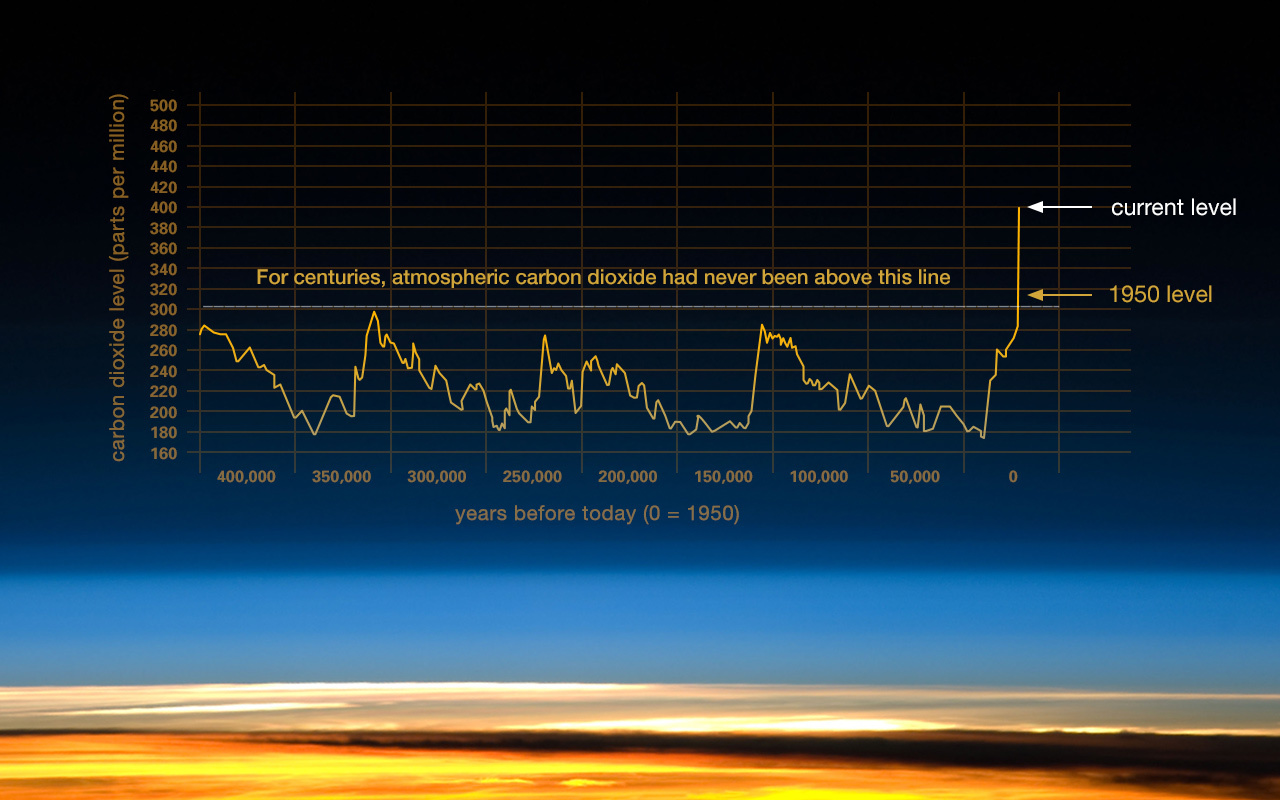
\includegraphics[width = .999\textwidth]{Figure/nasa_co2.jpeg}
\caption{This graph provides evidence that atmospheric CO2 has increased since the Industrial Revolution began. Image courtesy: https://climate.nasa.gov/evidence/}
\label{nasa_co2}
\end{figure}

\subsubsection{C. Conflicts and Wars}
An unbalanced energy distribution causes conflicts and wars. The wars, like Gulf War, are more or less derived from energy issues since WW2.\\

\subsubsection{D. Power Interruption}
With the use of unreliable electrical grids, power interruption occurs especially when a natural disaster, such as typhoon, earthquake, and wildfire, happens. Smart grids is more reliable than traditional grids. It’s possible to be build a dynamic technology, like Secondary Frequency Control (SFC), that grid operators need. Self-healing is possible when the storms hit, or physical attack occurs. Therefore, consumers will not encounter power interruptions.\\

\subsubsection{E. Equal Rights to Use Natural Power}
Everyone should have his/her right to use natural resources equally. However, in most countries, the fact is that a few large companies occupy the dominant position of public funds and gradually form a monopoly market. Entrepreneurs use their centralised power to restrict consumers’ right to disagree.\\

However, the technologies should start with the customers. It is connected with intelligent devices that always communicate with each other. The system creates and stores energy throughout the day and any extra energy flows back onto the grid to power neighbours and businesses. Those smart energy buildings then power entire communities. It’s distributed, clean, and more cost-effective.\\

\subsubsection{F. New Issues from Clean Energy}
Using clean energy from renewable resource could be one of the ways to solve the problems above! In fact, recently, California Assembly passed a bill requiring 100 percent of the state’s electricity to come from carbon-free sources by the end of 2045. In China and Germany, renewables are outgrowing their grids. The public is accepting the idea of using electric cars instead of fuel cars.\\

However, these renewable energy sources interfaced with national or state power systems will introduce new issues on stability, resilience, and reliability. Thus, power networks are under modification.\\

For countries like Switzerland, where 62\% of electricity comes from renewable sources, it’s another situation. Although it’s really friendly to the environment, energy instability has also increased. Sun doesn’t always shine, wind doesn’t always blow, and water doesn’t always flow.\\

\subsection{Solution: Secondary Frequency Control}
As these highly variable sources come to represent a growing portion of the grid, it becomes more and more important to develop an accurate and validated model to represent these units in the computational tools used to analyse the ancillary services of smart grids.\\

Smart grids will power the modern city, and Secondary Frequency Control is one of the most important parts in smart grids to ensure the energy security in electricity systems and to allow increasing renewable energy penetration\\

Secondary Frequency Control ensures that the frequency of the electricity network is always restored to its nominal value when disturbances occur in the system. The frequency is one of the key “health” indicators of smart grids. Actively monitoring and controlling it will ensure system security. This is done by remotely controlling the power output of generating units (both conventional and renewables) through a communication network.\\


\section{Thesis Outline}
This project consists of two parts — PART I Algorithm and PART II Test Case Scenario (Nordic).\\

PART I focuses on the task of understanding and building Secondary Frequency Control (SFC) model and PI control algorithm so that we are able to test our cases in PART II.\\


In Chapter 2, we give an overview of Frequency Control, including Primary Frequency Control (PFC), Secondary Frequency Control (SFC) and Tertiary Frequency Control (TFC). We discuss the emergency control with PFC, SFC and TFC.\\

In Chapter 3, we formally focus on the physical theory behind Secondary Frequency Control (SFC) which is the base of the whole project. We briefly discuss PID control and argue that we should use PI control to reduce the probability of risk. We then discuss how to build a communication layer on top of an existing smart grid simulator and design a centralised controller for stabilising the system. We describe the algorithm we built named sfc: its key parameters, tuning methodology, and some implementations. We finally define the acceptable results based on the official report from Nordic, and with that, we build our own analytical tools. With these tools, we can plot a 2D even a 3D diagram, find the eligible results and give feedback to our controller in PART II.\\

PART II views testing in a specific test case scenario (Nordic) as an important part such as the impact of different time delays. Detailedly,\\

In Chapter 4, we focus on testing the system in a low time delay. We discuss how to choose an appropriate generator as a breaker and how to tune the range of  gain. Before simulating, we predict some expected results based on the physical theory behind Secondary Frequency Control (SFC). Then we present a comprehensive evaluation on the simulation results. We describe the results and compare them with the expected one. We discuss why my prediction had deviation or missing. We discuss the risk, i.e. the rate of change of power, of the generators and how to remove unacceptable results. We will finally show a 2d plot and a simulation result.\\

In Chapter 5, we discuss the impact of different time delays. We increase the delay and use the range of gain in Chapter 4. We will explain why we think it is reasonable to continue using the range of gain in Chapter 4. In fact, it is logical forward-looking. Then we will predict the simulation results based on the physical theory behind Secondary Frequency Control (SFC) and the results in Chapter 4. Then we present a comprehensive evaluation on the complicated simulation results. We will describe the results with a plotted 3d graph. We will discuss some unpredictable results and some seemingly irregular data. We discuss the risk of the generators, like what we do in Chapter 4, and how to remove unacceptable results. We will finally show a 3d plot and a best simulation result.\\

In Chapter 6, we discuss the impact of generator size. We fix the size of gain and the size of  delay in this chapter and we discuss the reason for doing this. Differently, We only test g1, g3, g4, g5, g9, g10, g11, g12, g13 and g19 as breaker, the generator will disconnected from the grid as the only disturbing factor, based on Section 4.1.1. Before implementing, we predict some expected results based on Section 4.1.1 and understanding on energy and power. We analyse the results and they prove our prediction. We will see the relationship between the output and the size of a generator. We finally analyse if the system will have risk and the relationship between the size of a generator and the chance to have a risk. \\

In Chapter 7, we test Emergency Control and discuss the impact of different time delays without tuning gains. We will firstly define Emergency Control although we have discussed it in Chapter 2. We predict some results based on Secondary Frequency Control (SFC) and the conclusions in Chapter 4. After implementing and analysing the results, we will discuss why my predictions are “wrong”. We finally do a risk assessment for the system as we did before.\\

We will finally conclude in Chapter 8.\\

\section{Contributions}
The contributions of this thesis are summarised as follows:\\
\begin{itemize}
  \item We built a communication layer on top of an existing Smart Grid simulator and design a centralised controller for stabilising the system.\\
  
  \item We researched situations that cause disturbances, including generators interruption, high time delays and blackout. We built a series of efficient models for analysing the performance of the system and remove any unacceptable results. After hundreds of manual data proofreading, these models has demonstrated superior analytical ability.\\
  
  \item We built an optimal controller for stabilising the frequency based on the centralised controller and the analytical models above. This optimal controller has demonstrated superior performance of restoring frequency when disturbances occur in the system.\\
\end{itemize}


\part{Algorithm}
\chapter{An Overview of Frequency Control}
\label{chap:2}
\section{Overview}

Every country has its nominal frequency of the oscillations of alternating current in an electric power grid transmitted from a power station to the end-user. For instance, the nominal value is 50Hz in the UK while it’s 60Hz in USA.\\

However, if a load is suddenly connected or disconnected to the system, or if the protection equipment suddenly disconnects a generating, there will be a distortion in the power balance between that delivered by the turbines and that consumed by the loads. This imbalance is initially covered from the kinetic energy of rotating rotors of turbines, generators and motors and, as a result, the frequency in the system will change. \\

If there is a mismatch between the generation and the demand, for instance, due to the outage of one generating unit, then the frequency starts to drop down. \\

If no control is applied, the frequency largely deviates and then reaches a meagre and steady-state value, due to which the electrical grid is shut down.\\

\begin{figure}[htp]
\centering
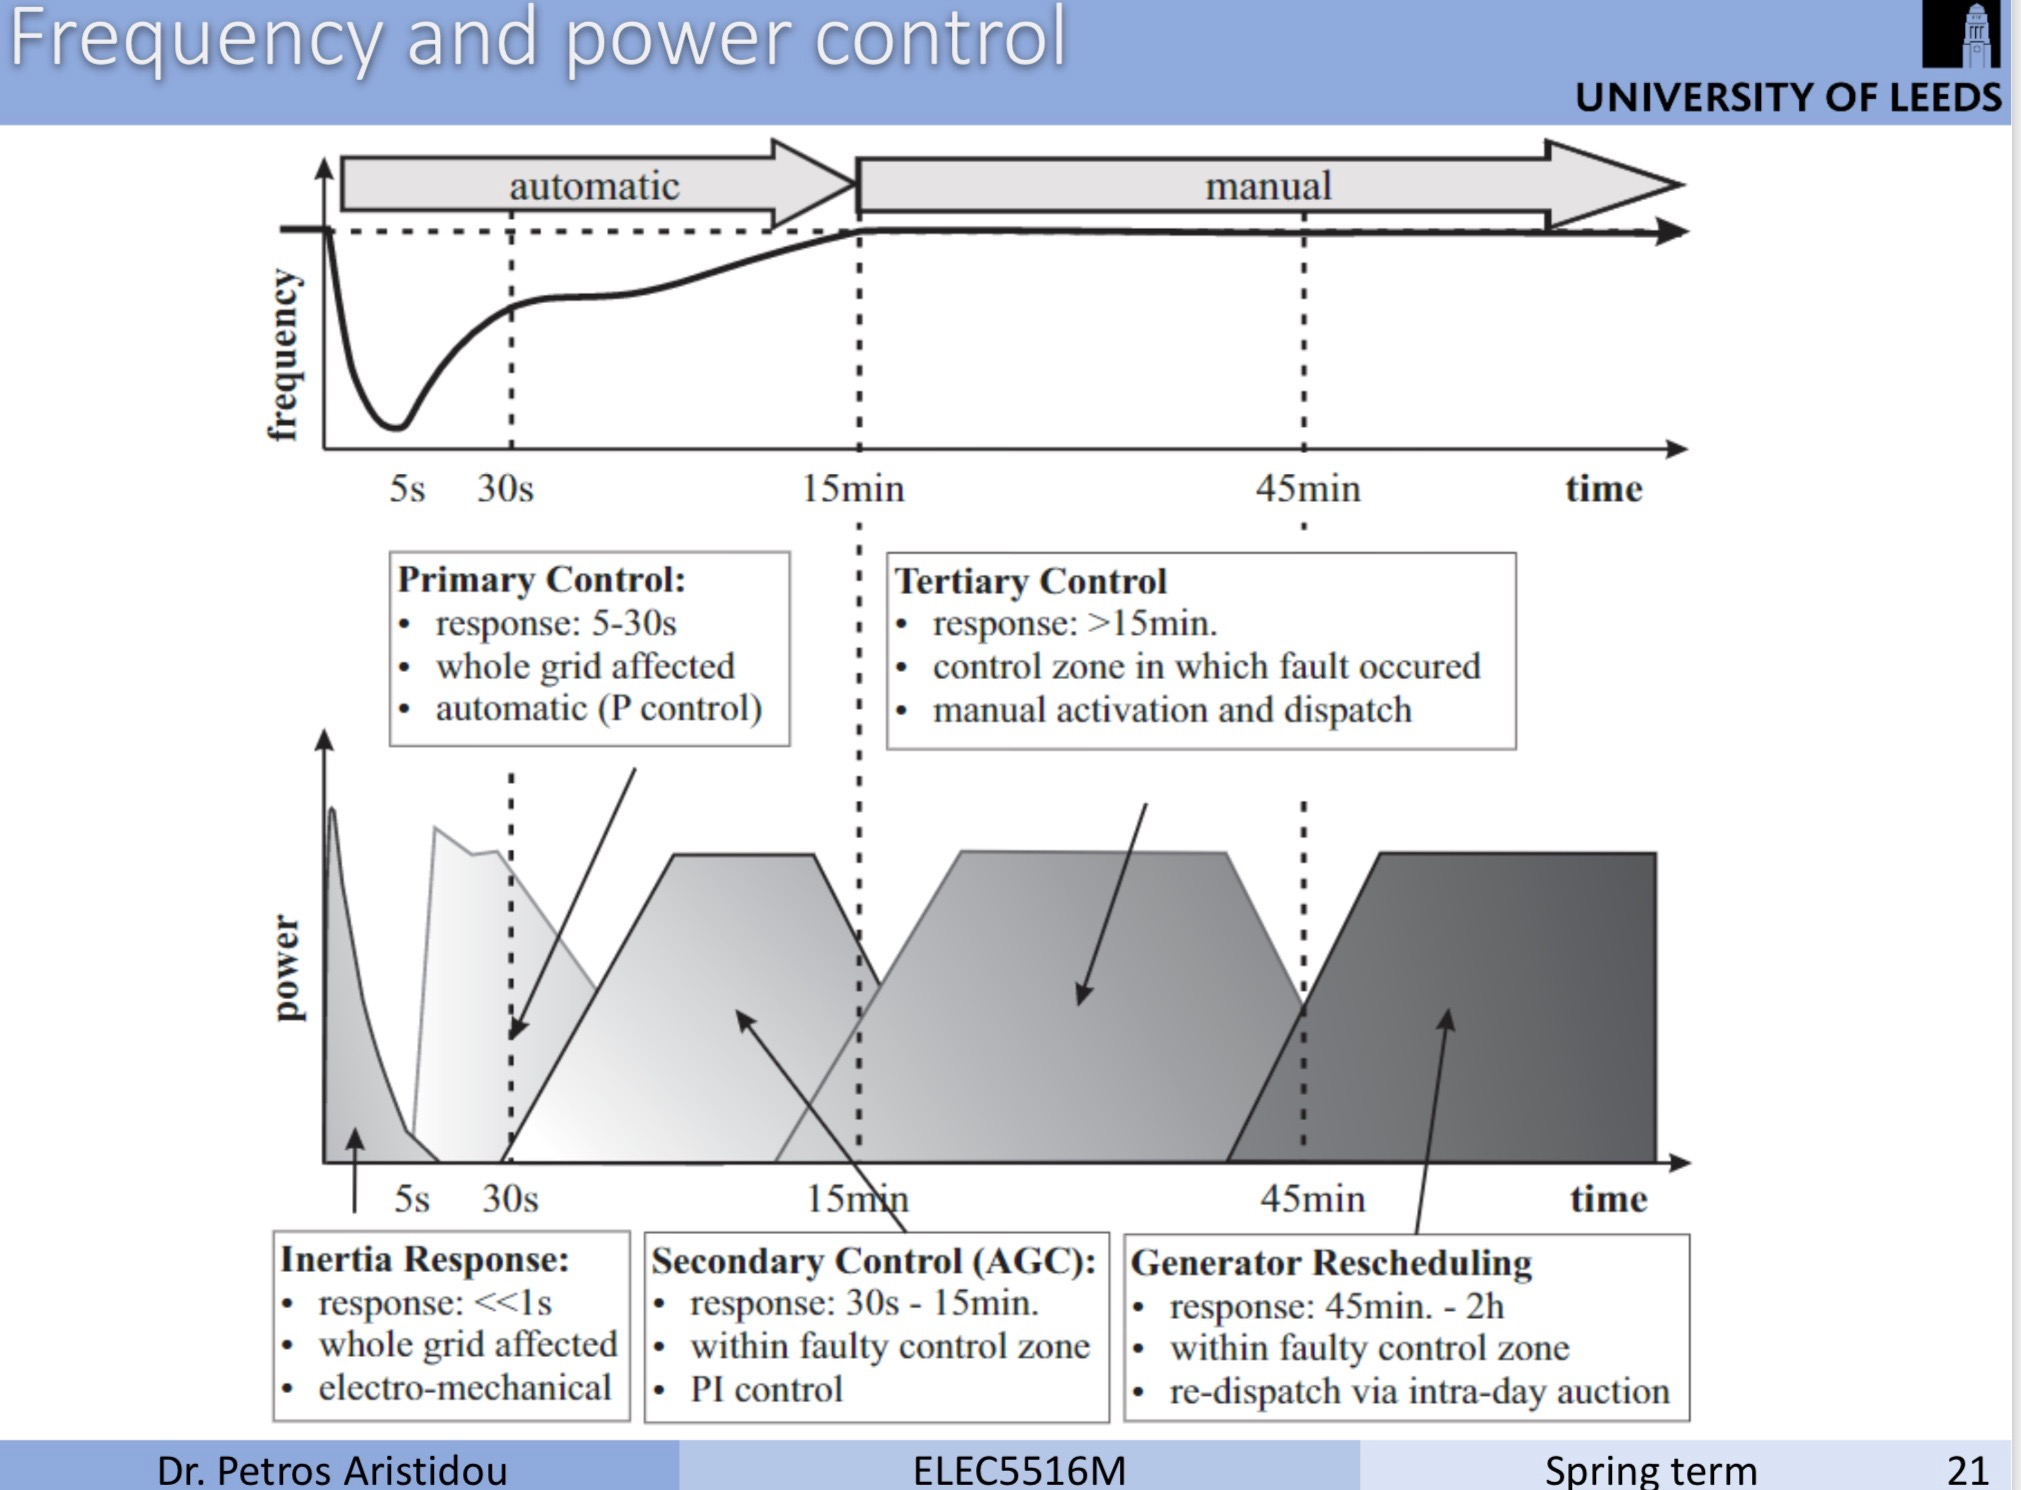
\includegraphics[width = .8\textwidth]{Figure/leeds_freq_control.jpeg}
\caption{Frequency and power control}
\label{leeds_freq_control}
\end{figure}

The mechanism of primary frequency control is to restore the active power balance in a power system. After primary control takes place, the power balance is restored at a lower or higher frequency. Normally it takes seconds and responses from 5 seconds to 30 seconds. It is a partly Automatic Generation Control.\\


However, the frequency does not go back to its nominal value and remains at a steady-state value below or above the nominal one. To avoid damages to equipment and loads, we need secondary frequency control to restore the frequency balance to its nominal value or to eliminate the steady-state error/frequency error. Normally it takes minutes and responses from 30 seconds to 15 minutes. It is a fully Automatic Generation Control.\\


Tertiary Frequency Control encompasses actions taken to capture current and future emergencies by getting resources. Alternate deployment and recovery after a disturbance are common types of Tertiary Control. Normally it takes dozens of minutes and responses longer than 15 minutes. It is a fully manual control.



\chapter{PID Control Algorithm}
\section{The physical theory behind Secondary Frequency Control}
From Chapter 2, we mentioned that disturbances occur in the system, there will be a distortion in the power balance between that delivered by the turbines and that consumed by the loads. The imbalance is from the kinetic energy of rotating rotors of turbines, generators and motors and, thus, the frequency in the system will change. If no control is applied, the frequency largely deviates and then reaches a meagre and steady-state value, due to which the electrical grid is shut down. \\

We also mentioned that the system will firstly starts Primary Frequency Control and the frequency will remains at a steady-state value below or above the nominal one. After that, Secondary Frequency Control starts.\\

The mechanism of Secondary Frequency Control is to restore the frequency to the nominal one.\\

Secondary frequency control, or load frequency control (LFC), or automatic generation control (AGC), is an automatic control that restores the frequency back to its nominal value in a centralised way. It's implemented that is activated after the primary frequency control. Typically, it takes 30 seconds to 15 minutes.\\

\begin{figure}[htb]
\centering
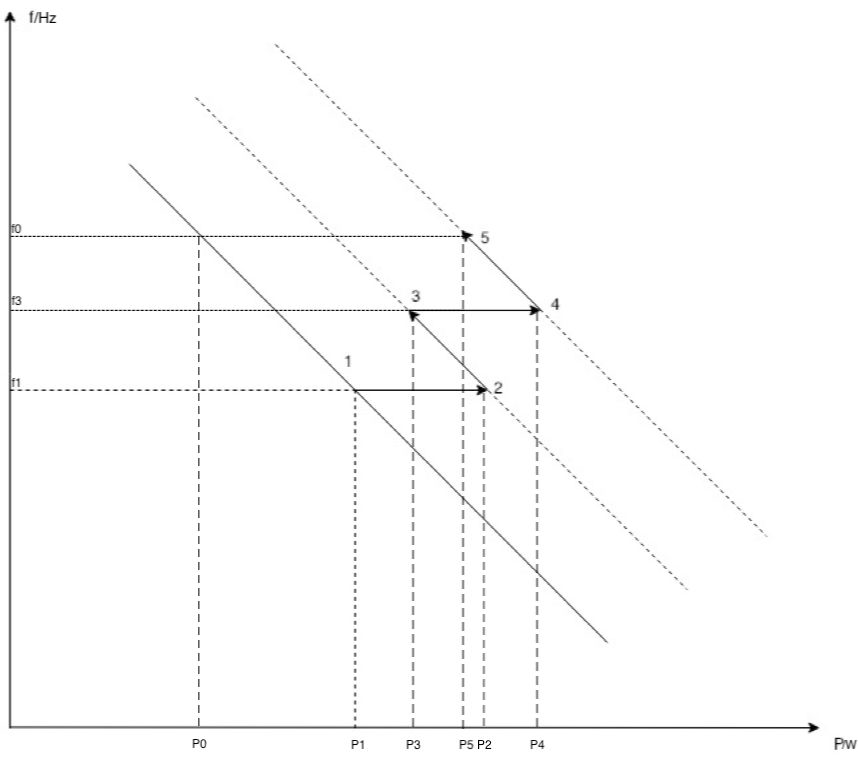
\includegraphics[width = .5\textwidth]{Figure/theory_sfc.png}
\caption{Equilibrium points for an increase in the power demand.}
\label{theory_sfc}
\end{figure}

According to Figure \ref{theory_sfc}, frequency value will rise as reference power rises. Assumed that point 1 is the situation after primary frequency control happens and point 5 has the nominal value of frequency. When trying to raise the reference power a little bit, point 1 will shift to point 2. Due to the power rise, the frequency of the system will rise, so point 2 will move to point 3. Changing more reference power of individual governors will move the overall generation characteristic of the system upwards. Eventually, this will lead to the restoration of the rated frequency (f0).\\

\begin{figure}[htb]
\centering
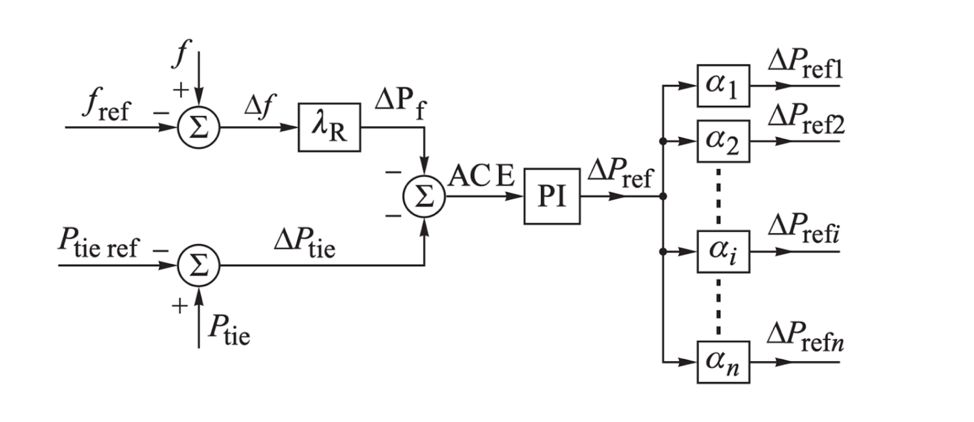
\includegraphics[width = .618\textwidth]{Figure/agc_blockDiagram.png}
\caption{Functional diagram of a central regulator.}
\label{agc_blockDiagram}
\end{figure}

As seen in Figure \ref{agc_blockDiagram}, the frequency (f) will be measured in the local network and compared with the reference frequency to produce an amplified signal ( ∆P f ) that is proportional to the frequency deviation (∆f). For instance, if the frequency is smaller the reference frequency, then the signal ∆P f will be negative. Thus, input signal ACE is positive according to the functional diagram. Therefore, output signal ∆P ref is positive and it will adjust the system by raising the reference value of the power. Then the system will have a new frequency value ( f new ) that will go through the functional diagram again to compare the difference with the value of the reference frequency. ACE won’t be zero and the frequency won’t be stopped adding until we remove any error.\\

In this standard case, which ignores the existence of tie-line interchange error, the only condition to remove errors is the frequency deviation (∆f) equals to zero.\\

\begin{figure}[htb]
\centering
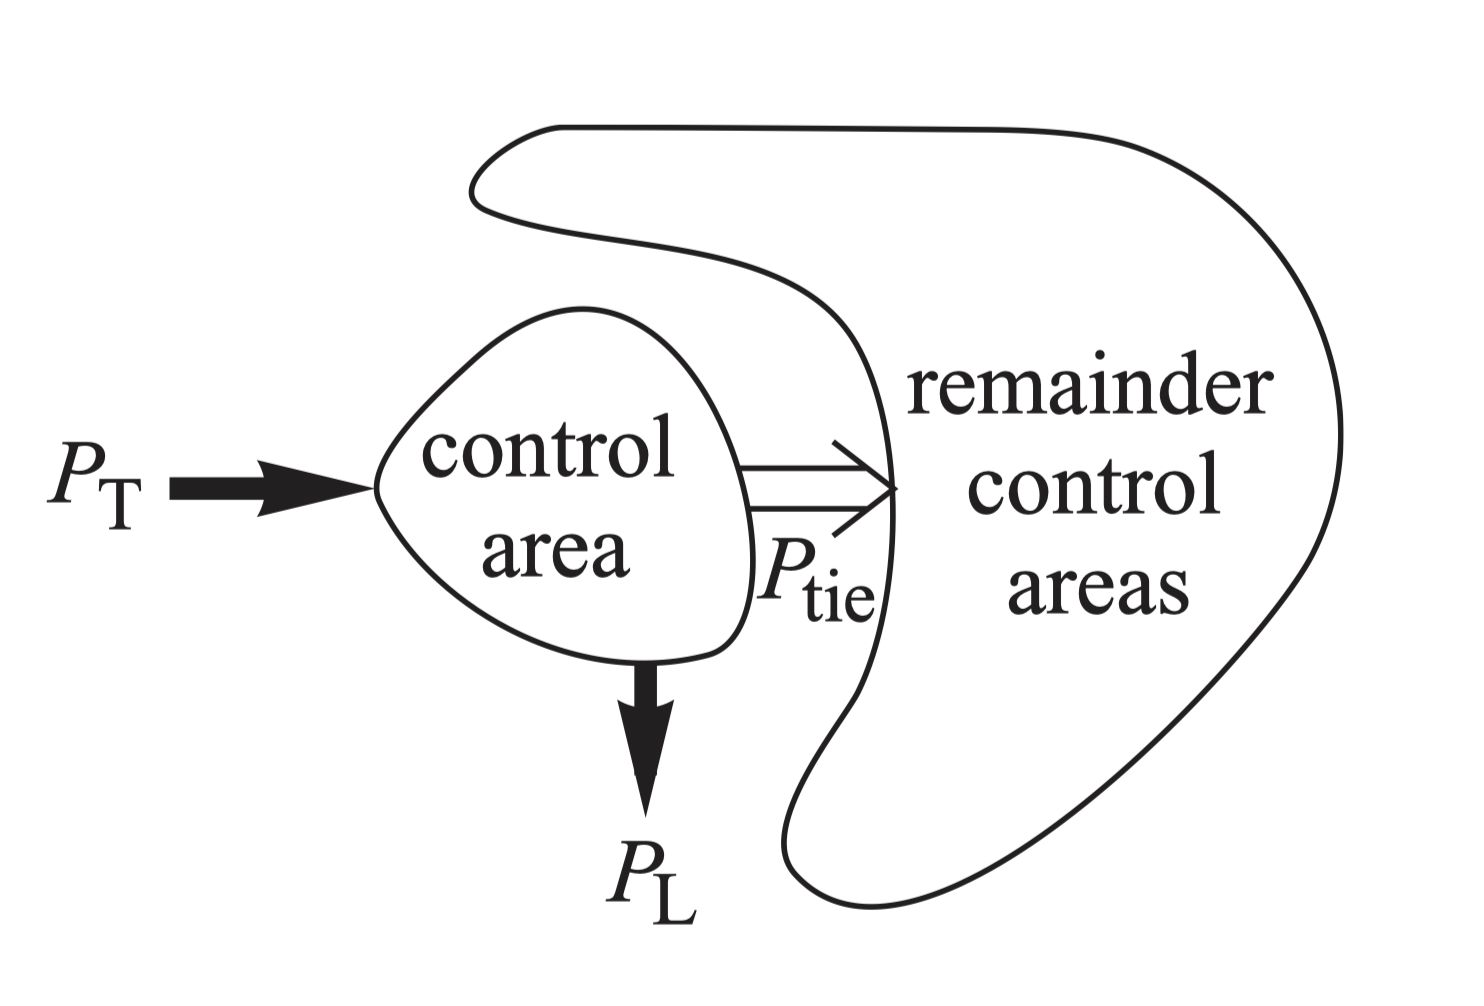
\includegraphics[width = .618\textwidth]{Figure/controller_powerBalance.png}
\caption{Power balance of a control area.}
\label{controller_powerBalance}
\end{figure}

However, it would be more difficult if consider the situation of tie-line interchange error. In interconnected power systems, AGC is implemented in a way where each subsystem has its own regulator. As shown in Figure \ref{controller_powerBalance}, the power system is in equilibrium if the total power generation ( P T ), the total power demand ( P L ) and the net tie-line interchange power ( P tie ) satisfy the condition in each subsystem:\\
P T − (P L + P tie ) = 0.\\

The objective of each regulator of the subsystem is to maintain frequency at the nominal level and to maintain net tie-line interchanges from the given area at the scheduled values. If there is a disturbance in one subsystem, then regulators in each subsystem should try to restore the frequency and net tie-line interchanges. Each subsystem regulator should enforce an increased generation covering its own area power imbalance and maintain planned net tie-line interchanges.\\

As shown in Figure \ref{agc_blockDiagram}, to obtain a signal proportional to the tie-line interchange error ( ∆P tie ), the information on power flows in the tie-lines is sent via telecommunication lines to the central regulator which compares it with the reference value. Then the signal ( ∆P f ) is added to the net tie-line interchange error ( ∆P tie ) so that ACE is: \\

ACE =− ∆P f − ∆P tie .\\

The situation here is similar to the situation above, where we ignore tie-line interchange error, except for the condition to remove errors. In this book [4], it shows us zeroing of errors can be achieved in two ways: zeroing of both errors ( P tie = 0 and f = 0) and achieving a compromise between the errors ( ∆P f + P tie = 0 or P f =− ∆P tie ).\\











\appendix
\chapter{}
...
%\bibliographystyle{plain}
%\bibliography{mybib}

\end{document}